\chapter{Appendix: Usage Guide}

This appendix summarizes the usage instructions from the AnDriDemo GitHub README. The repository is available at \url{https://github.com/ZeeChee-Guo/AndriDemo}.

\section{Upload Data}

The user first opens \url{http://localhost:5000/}. The system allows the user to choose one of the example datasets or upload a user's dataset. The user can also set the parameter \(\theta\), which represents the maximum allowed proportion of outliers.
\begin{figure}[H]
    \centering
    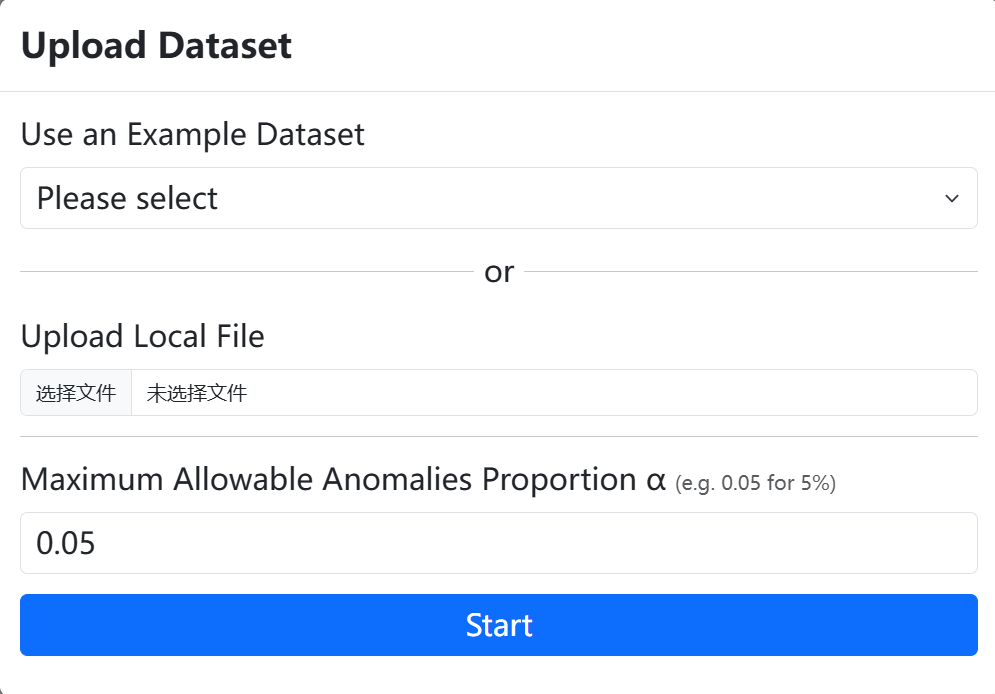
\includegraphics[width=0.85\textwidth]{figures/uploadDataset.png}
    \caption{Dataset upload.}
    \label{fig1}
\end{figure}

\section{Select Training Sets}

After loading the data, the user selects one or more training regions from the time-series chart. The upper chart is used for navigation, while the lower chart is for adjusting the size and position of the selected training set.

\begin{figure}[H]
    \centering
    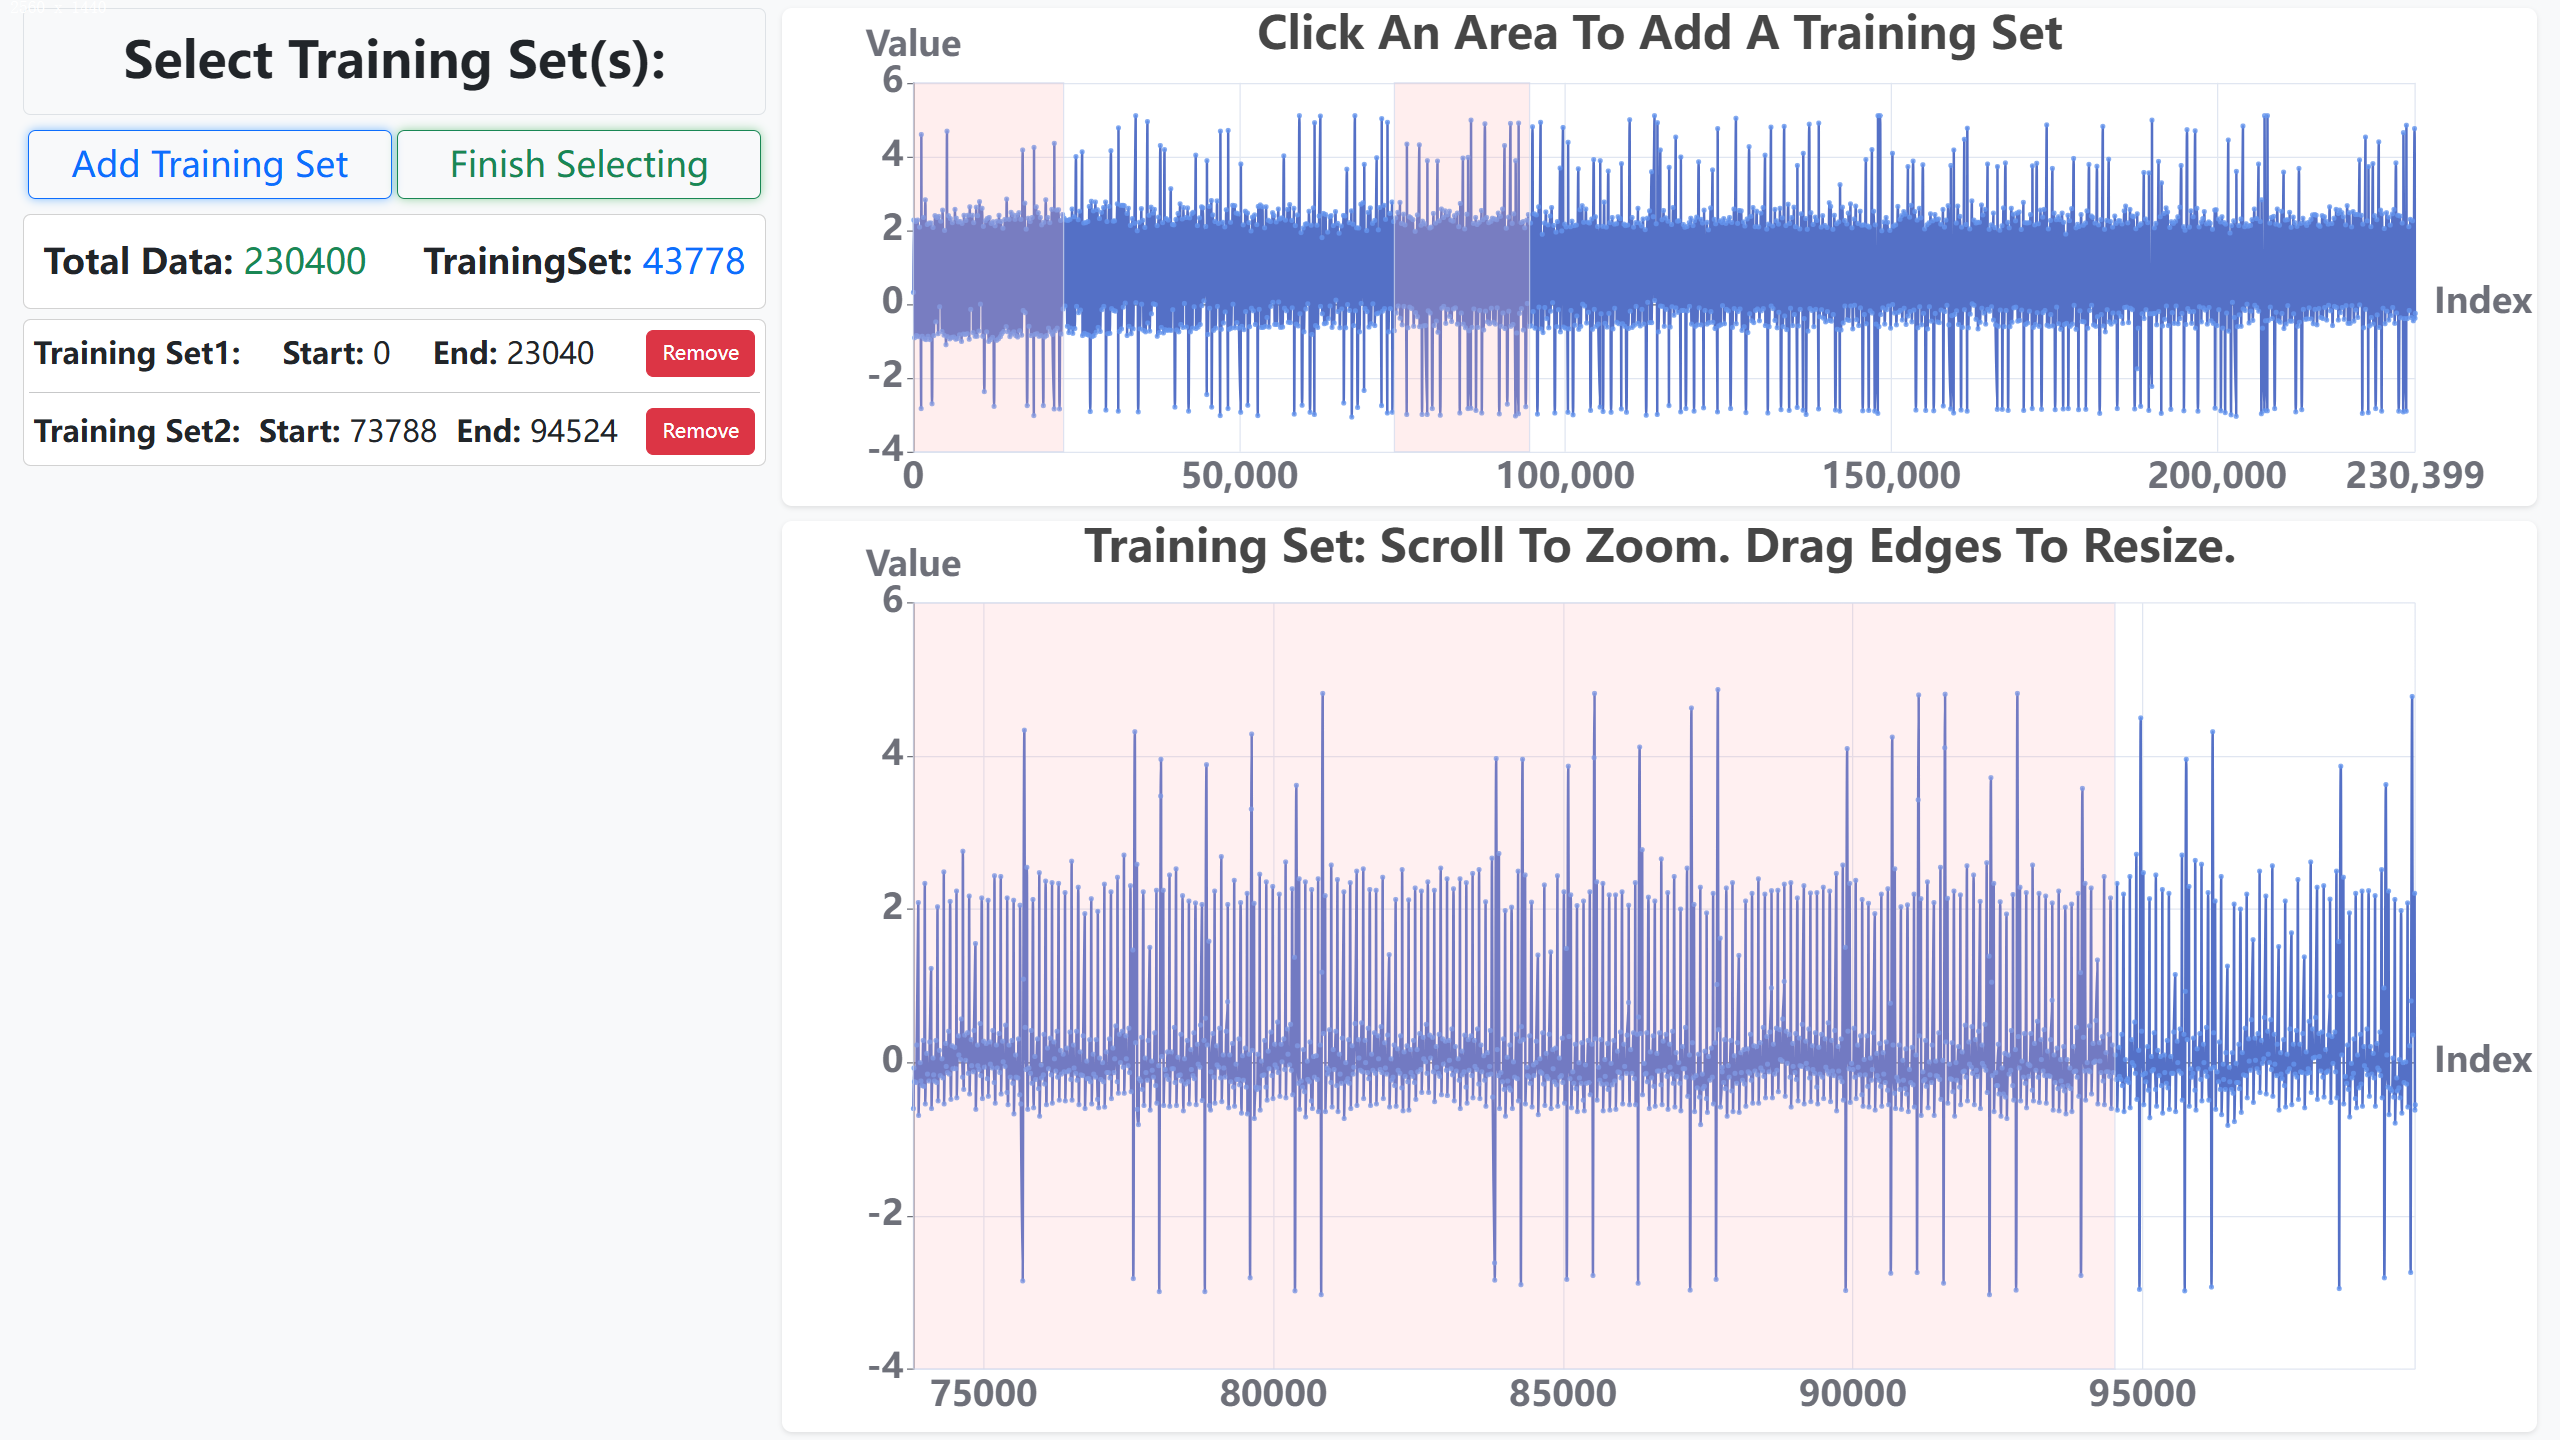
\includegraphics[width=\textwidth]{figures/selectTrainingSet2.png}
    \caption{Training-set selection.}
    \label{fig2}
\end{figure}

\section{Mark Anomalies}

The user can inspect the time series and mark abnormal regions interactively. The upper chart provides an overview and navigation control, while the lower chart is used to select specific abnormal points or regions.

\begin{figure}[H]
    \centering
    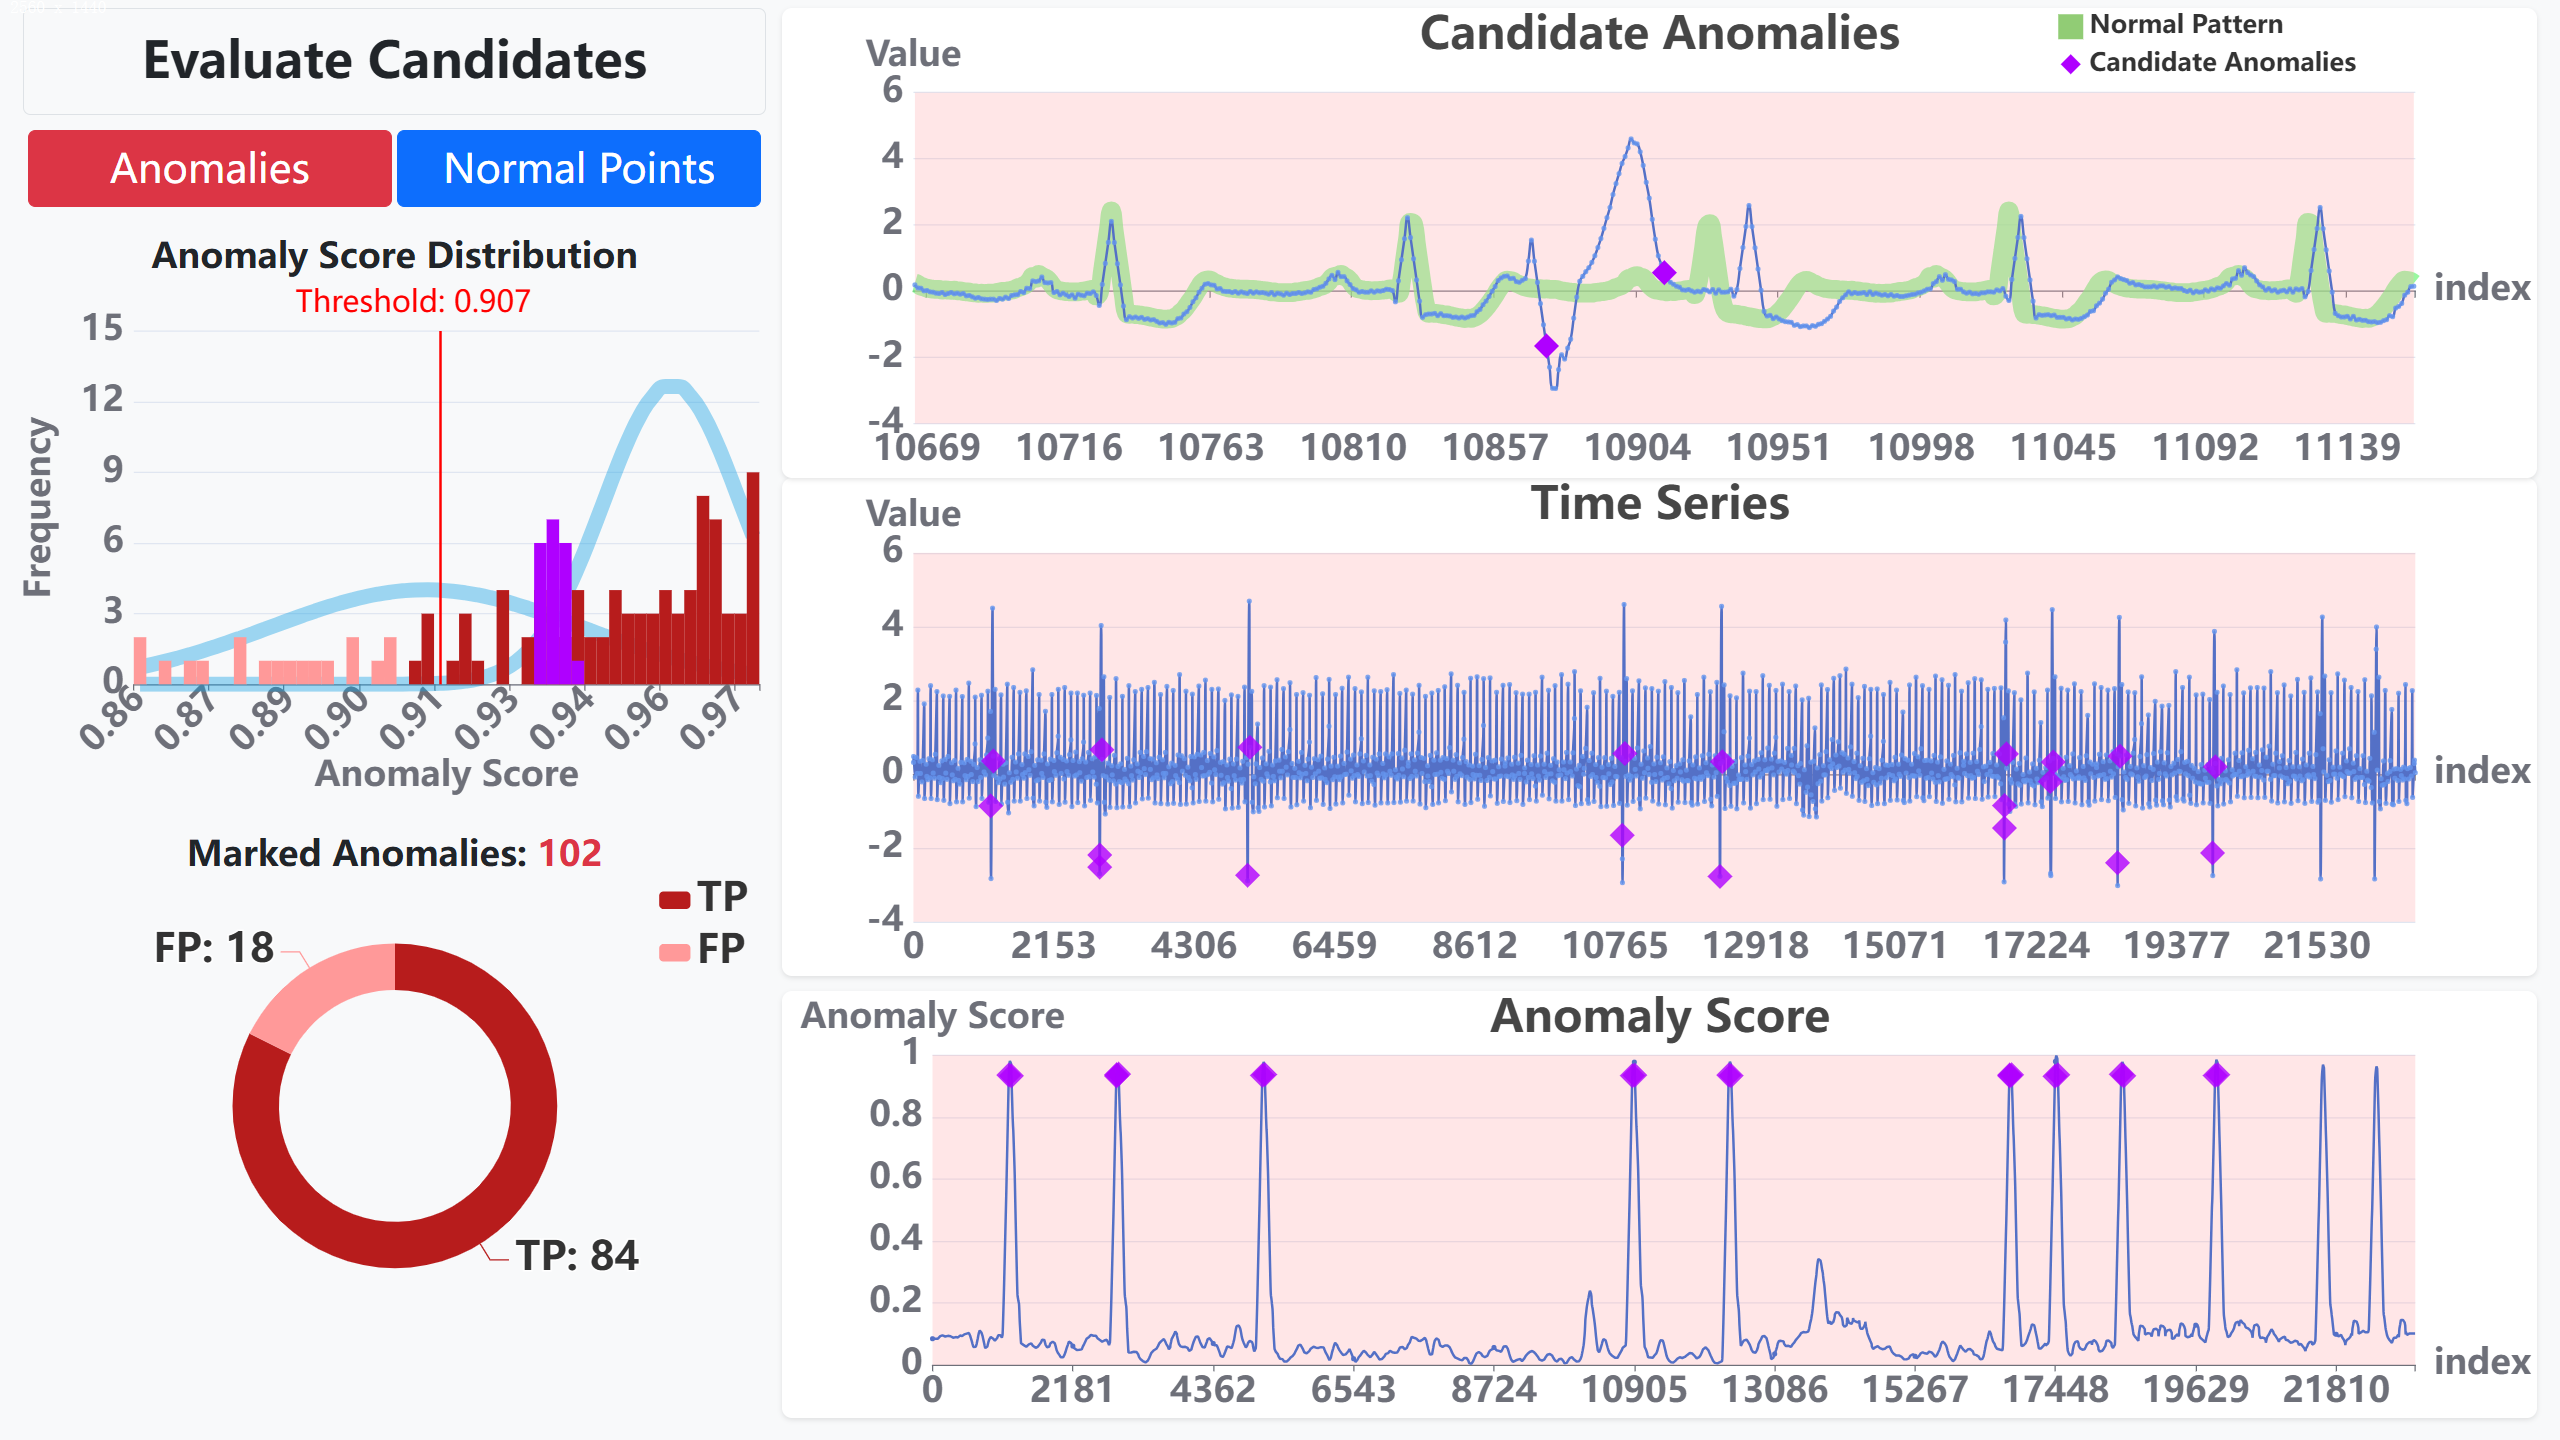
\includegraphics[width=\textwidth]{figures/markMoreLabels.png}
    \caption{Interactive anomaly marking interface.}
    \label{fig3}
\end{figure}

\section{Evaluate Points}

After the initial results are generated, the system presents candidate points for user evaluation. Based on the displayed normal patterns and related information, the user can determine whether selected points should be anomalies or normal points.

\begin{figure}[H]
    \centering
    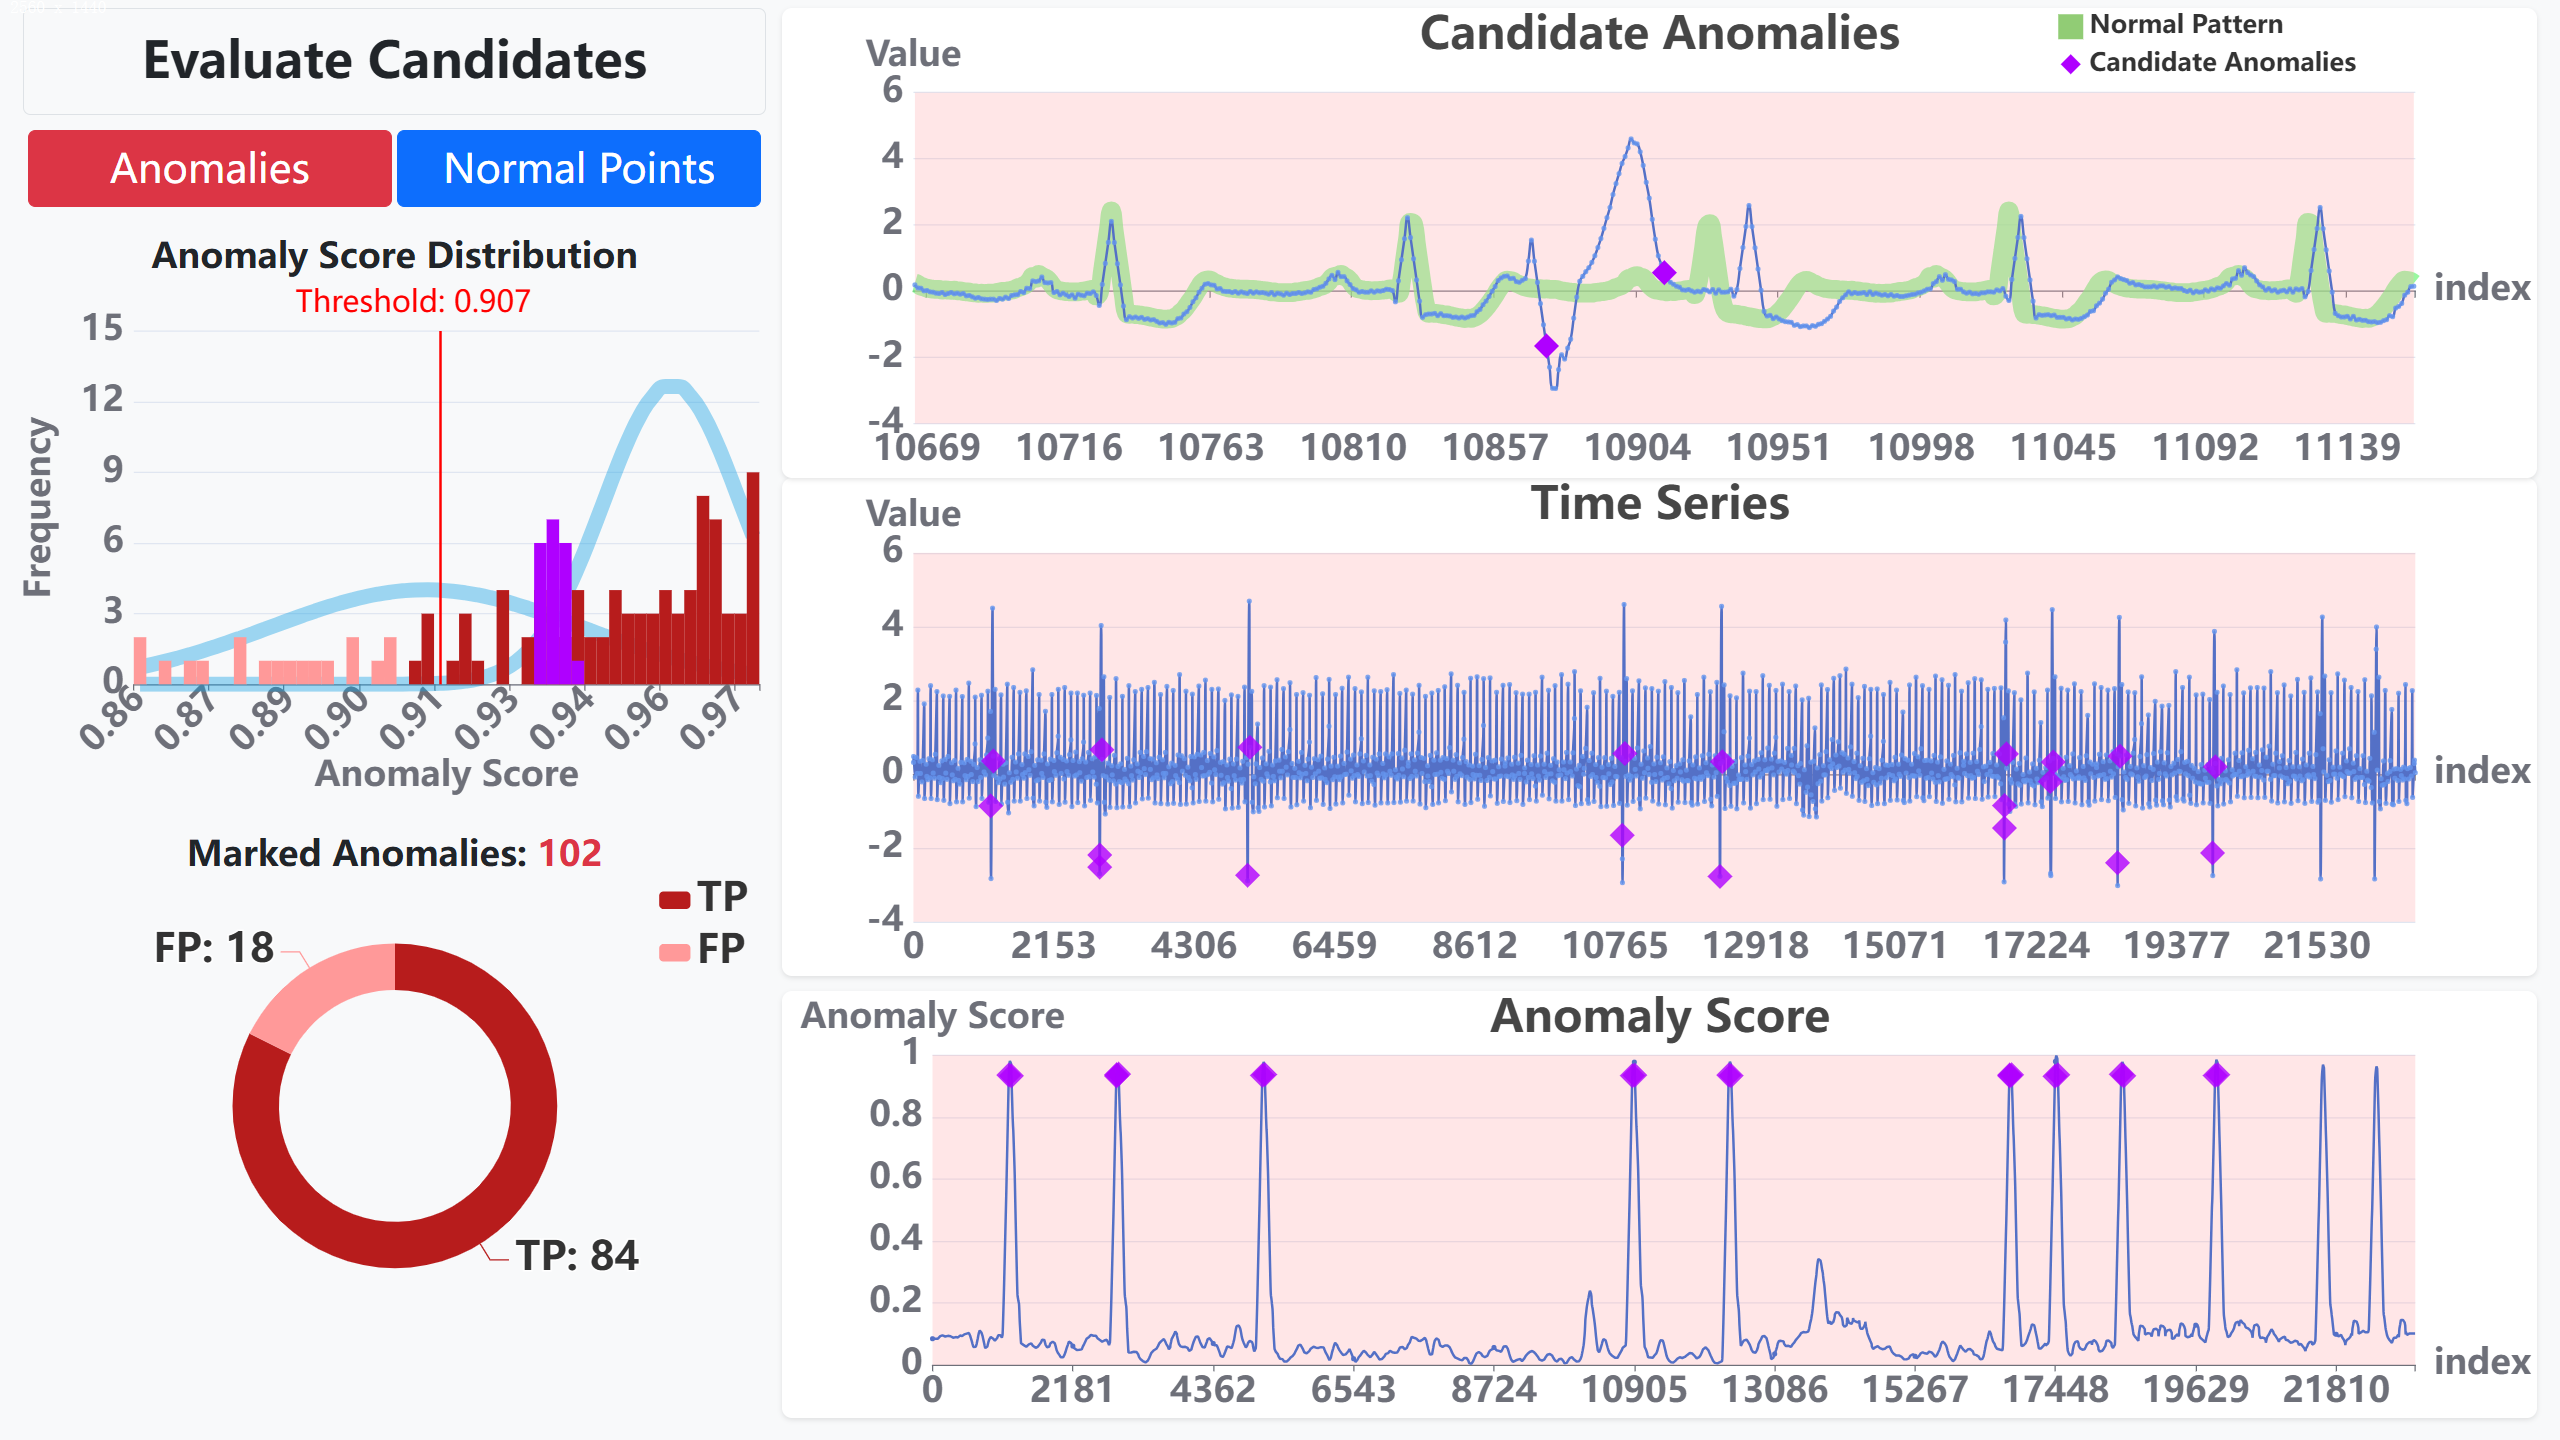
\includegraphics[width=\textwidth]{figures/markMoreLabels.png}
    \caption{Candidate-point evaluation interface.}
    \label{fig5}
\end{figure}


\section{Repeat With Other Algorithms}
The user can switch to other algorithms through the tab bar and repeat the active-learning workflow. This allows the user to compare threshold selection and labeling behavior across AnDri and baseline methods.

\section{View Results}

Finally, the user reviews the detection results and compares the accuracy of each algorithm. This result view helps explain why AnDri performs differently from the baselines under time-series drift.
\begin{figure}[H]
    \centering
    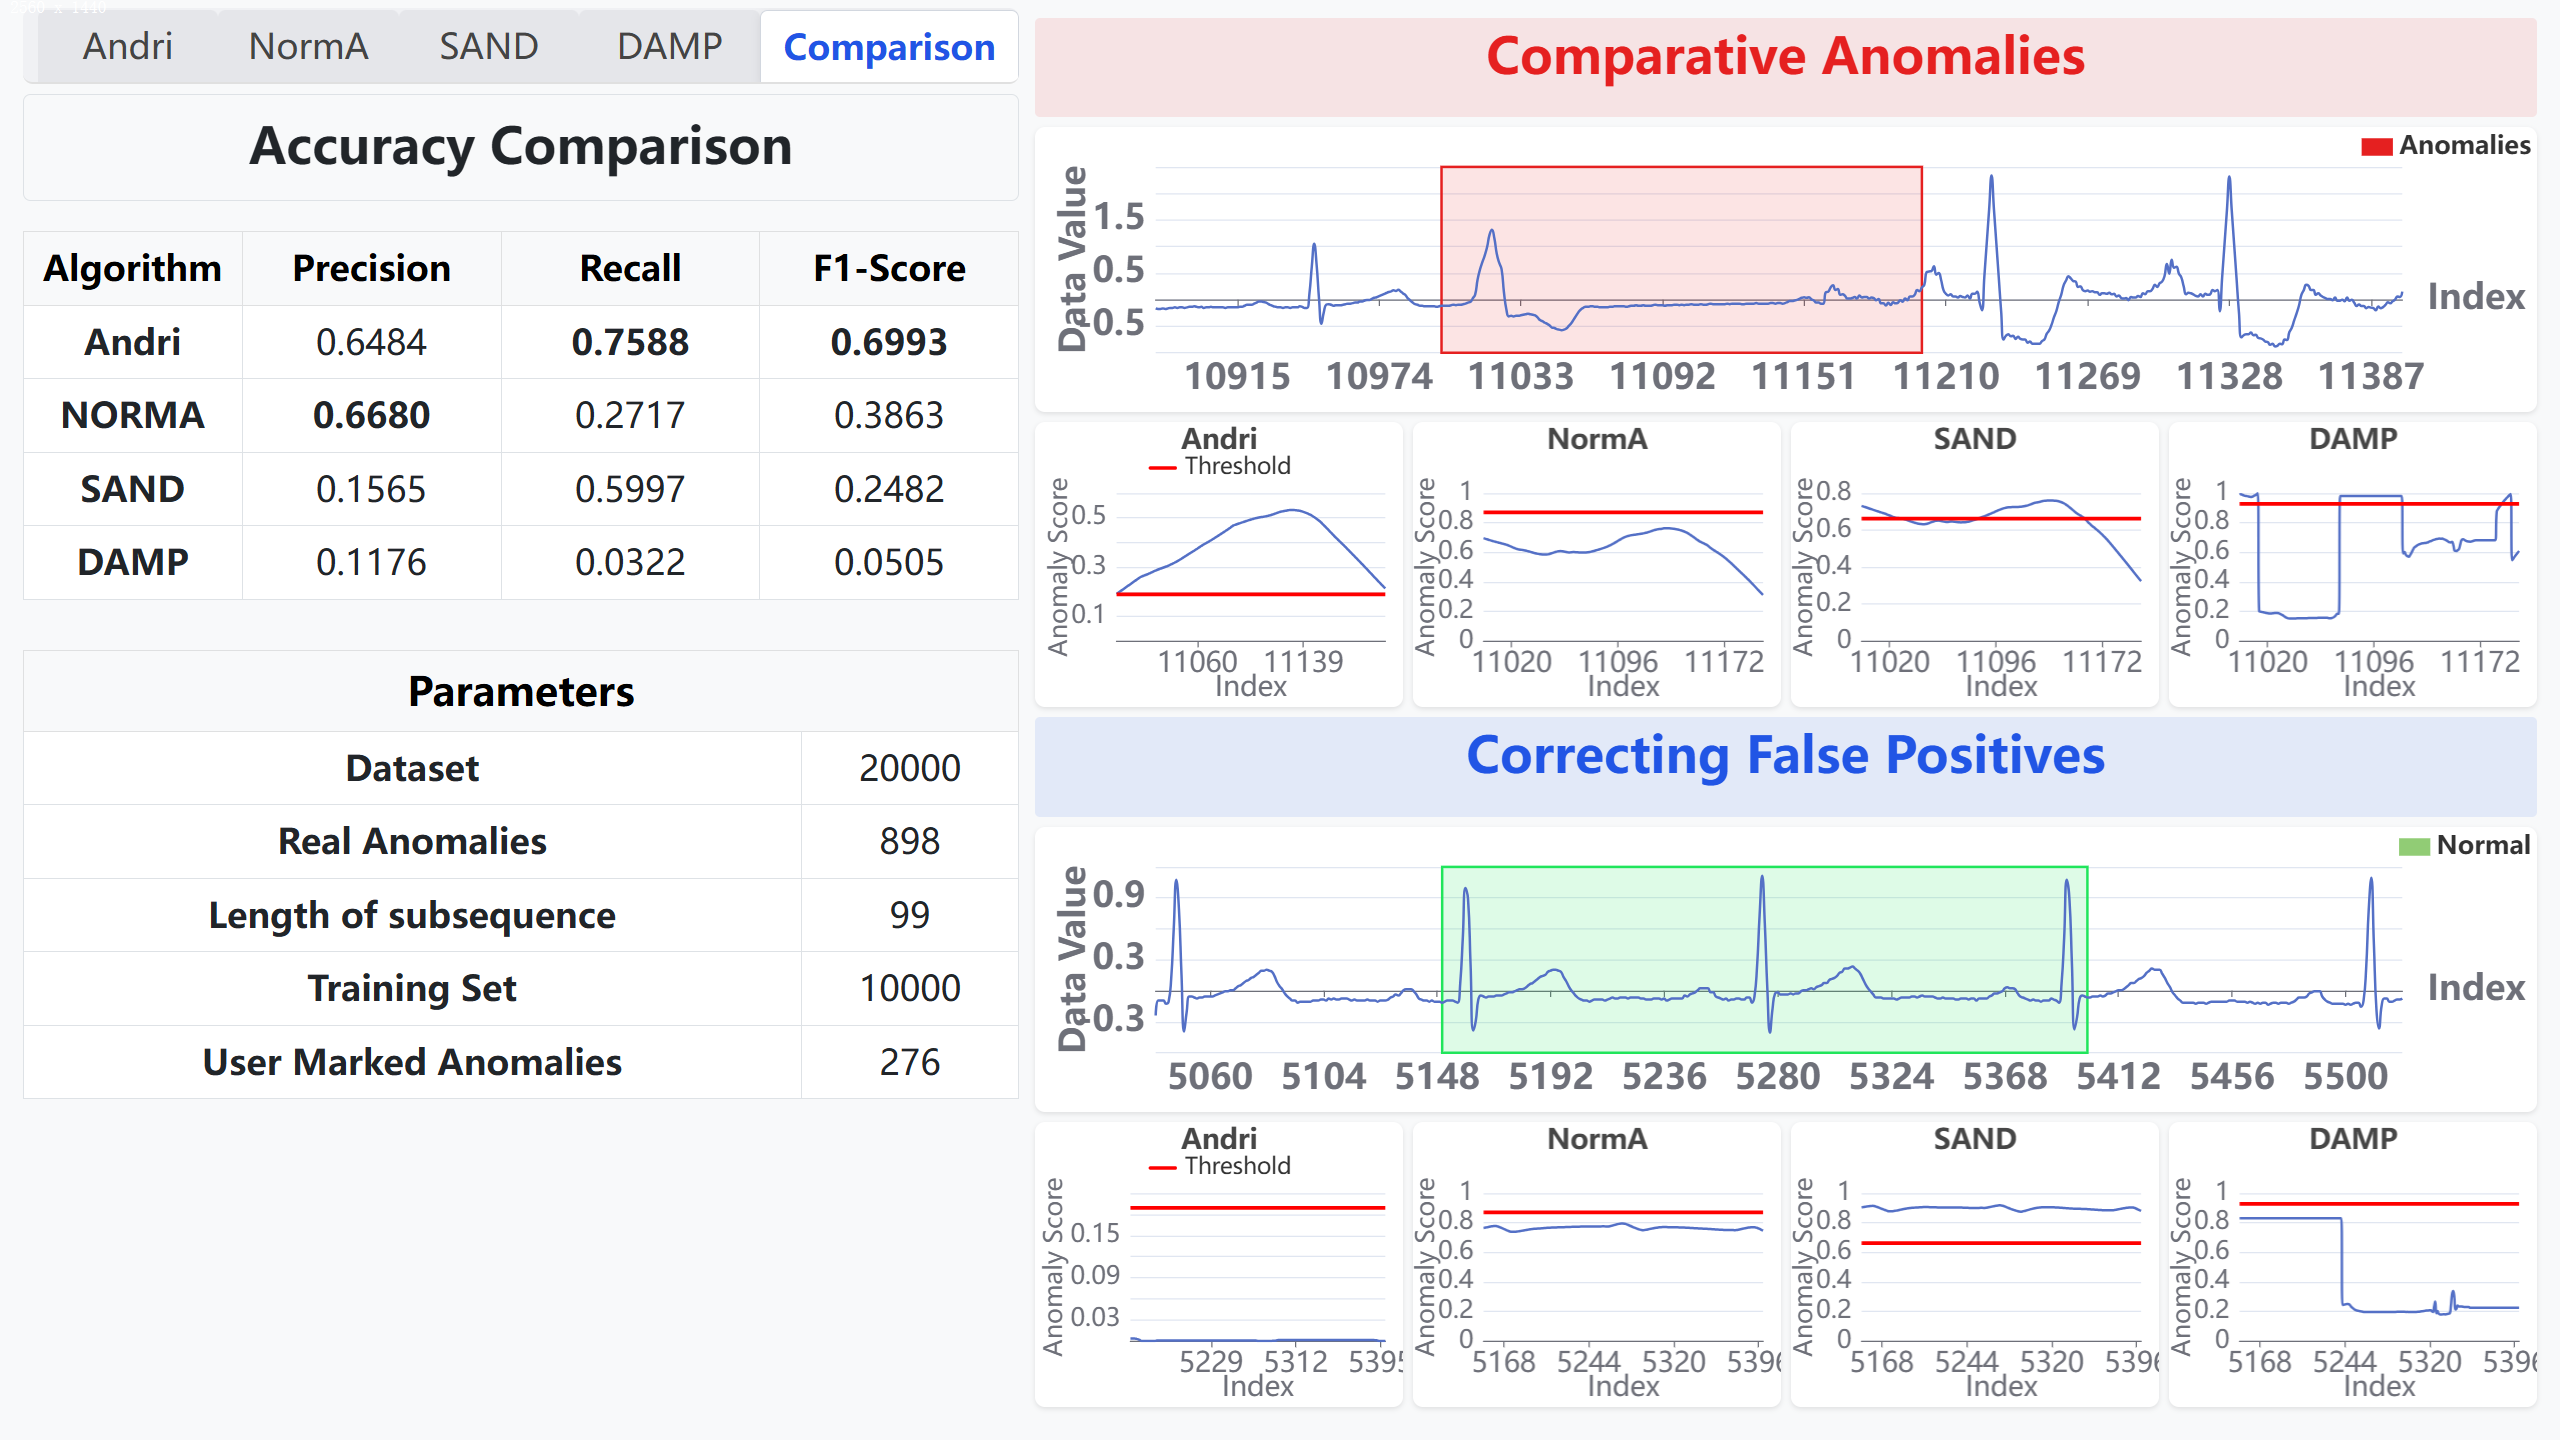
\includegraphics[width=\textwidth]{figures/andri_result.png}
    \caption{Result-review interface.}
    \label{fig6}
\end{figure}